% 图 49.3 —— 由 `checks/emit_hand.py` 自动拼出（probe 精测 + prims2 图元分解）
%%
% ⚠ 这是**稿子不是成品**：跑 `checks/checkhand.py 49.3` 看指标 + 看叠合图。
%%
%% ⚠ 待核：
%   · 本图 probe 报出阴影族 1 个 —— **本脚本不生成阴影**（要照原书手写）；prims2 的 strokes 里可能含阴影线，核对时留意别画重
%   · 可疑字形 1 项（空心圈 ⊙ 常被认成字母 o）—— 见文件末
%%
\documentclass[12pt]{standalone}
\usepackage{fontspec}
\setsansfont{Arial}
\newfontfamily\mfallback{DejaVu Sans}
\usepackage{tikz}
\begin{document}
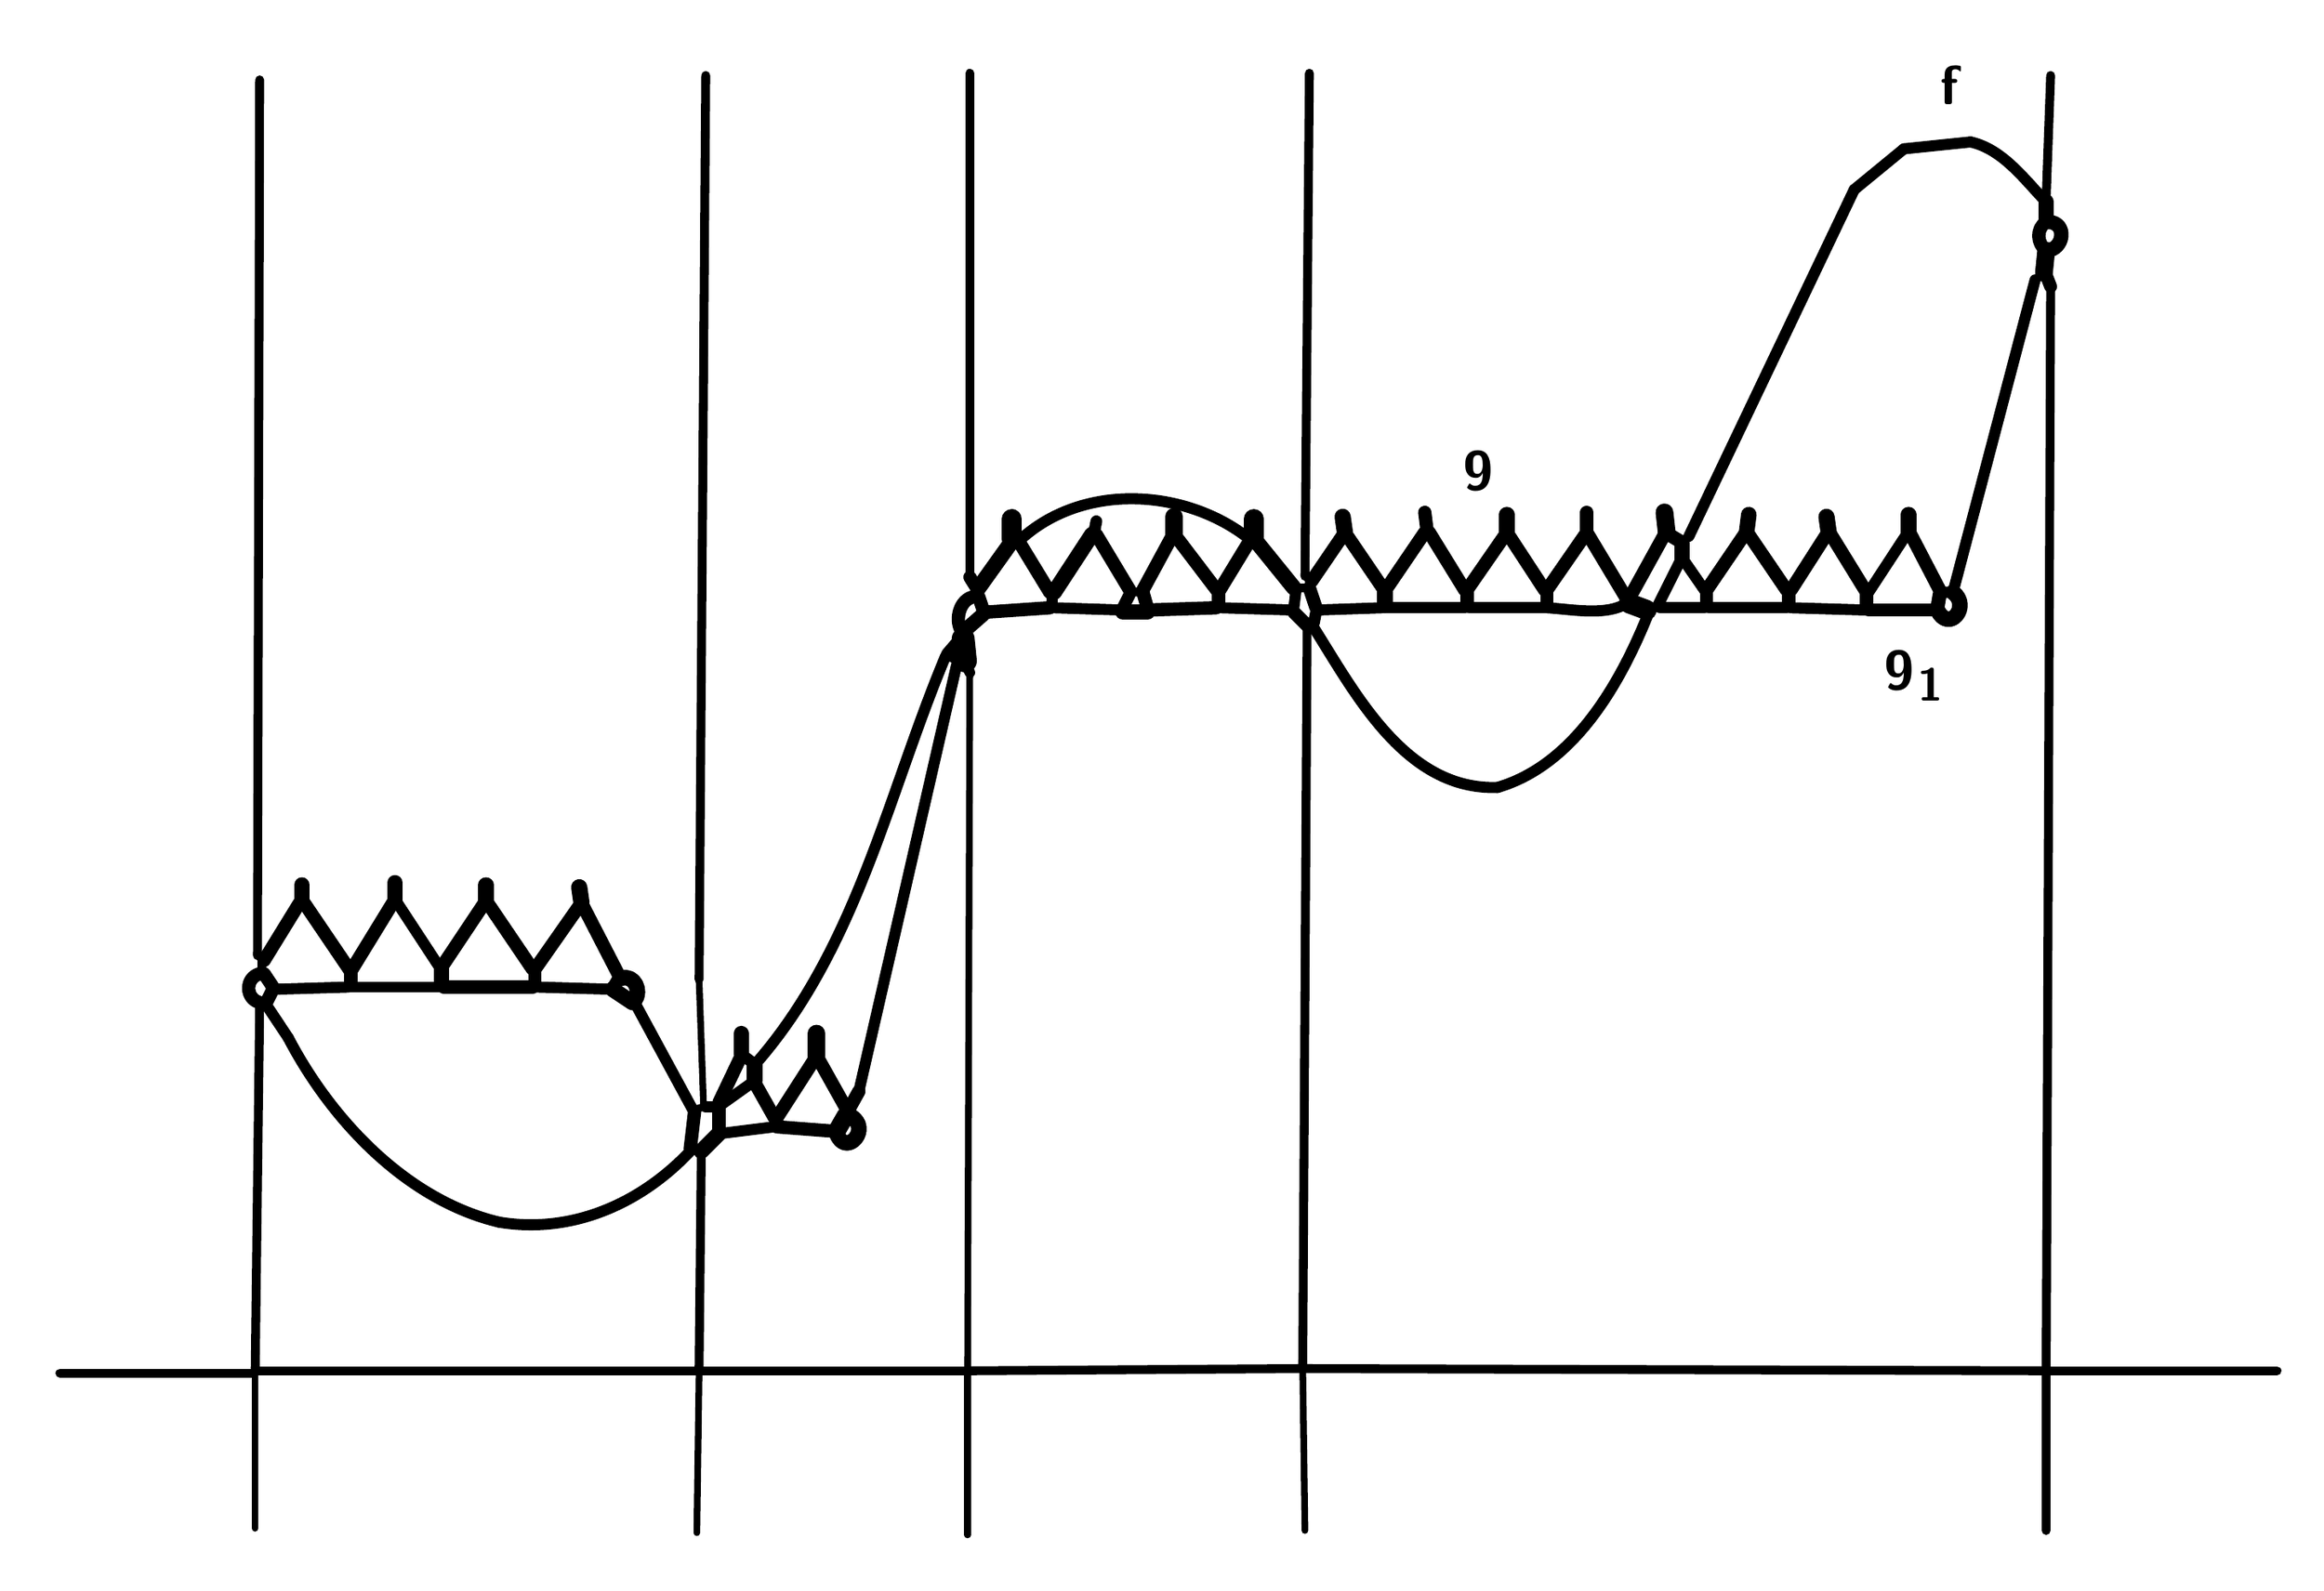
\begin{tikzpicture}[x=1pt, y=-1pt, line width=6.0pt, line cap=round, line join=round]

  %% ════ 直线段（prims2 的 strokes）════
  \draw[line width=6.0pt] (613.0,255.0) -- (596.0,230.0);
  \draw[line width=6.0pt] (813.0,231.0) -- (797.0,256.0);
  \draw[line width=7.0pt] (324.0,465.0) -- (324.0,456.0);
  \draw[line width=6.0pt] (705.0,230.0) -- (705.0,221.0);
  \draw[line width=6.0pt] (705.0,230.0) -- (687.0,256.0);
  \draw[line width=6.0pt] (705.0,230.0) -- (723.0,260.0);
  \draw[line width=3.0pt] (426.0,607.0) -- (427.0,293.2);
  \draw[line width=4.8pt] (427.0,293.2) -- (425.0,289.0);
  \draw[line width=6.0pt] (230.0,427.0) -- (209.0,396.0);
  \draw[line width=7.0pt] (446.0,234.0) -- (431.0,255.0);
  \draw[line width=6.0pt] (433.0,265.0) -- (431.0,259.0);
  \draw[line width=5.0pt] (188.0,435.0) -- (148.0,435.0);
  \draw[line width=6.0pt] (372.0,491.0) -- (358.0,466.0);
  \draw[line width=6.0pt] (372.0,491.0) -- (377.0,482.0);
  \draw[line width=5.0pt] (377.0,482.0) -- (421.0,290.0);
  \draw[line width=7.0pt] (189.0,427.0) -- (189.0,434.0);
  \draw[line width=5.0pt] (738.0,264.0) -- (758.0,264.0);
  \draw[line width=7.3pt] (813.0,223.0) -- (814.0,230.0);
  \draw[line width=4.0pt] (911.0,608.0) -- (578.0,607.0);
  \draw[line width=5.0pt] (313.0,489.0) -- (308.0,489.0);
  \draw[line width=6.0pt] (109.0,429.0) -- (113.0,435.0);
  \draw[line width=6.0pt] (864.0,256.0) -- (851.0,231.0);
  \draw[line width=6.0pt] (553.0,234.0) -- (539.0,257.0);
  \draw[line width=7.0pt] (496.0,266.0) -- (507.0,266.0);
  \draw[line width=3.0pt] (307.0,488.0) -- (305.0,431.6);
  \draw[line width=4.0pt] (305.0,431.6) -- (308.0,24.0);
  \draw[line width=3.8pt] (910.0,114.0) -- (907.0,116.2);
  \draw[line width=5.0pt] (907.0,116.2) -- (870.0,257.0);
  \draw[line width=5.0pt] (737.0,263.0) -- (747.0,243.0);
  \draw[line width=5.2pt] (329.0,469.0) -- (325.0,466.0);
  \draw[line width=4.0pt] (106.0,608.0) -- (304.0,608.0);
  \draw[line width=6.0pt] (148.0,428.0) -- (127.0,397.0);
  \draw[line width=6.0pt] (148.0,428.0) -- (167.0,397.0);
  \draw[line width=6.0pt] (148.0,428.0) -- (148.0,434.0);
  \draw[line width=8.0pt] (740.0,221.0) -- (741.0,230.0);
  \draw[line width=5.0pt] (749.0,243.0) -- (758.0,256.0);
  \draw[line width=6.0pt] (508.0,265.0) -- (538.0,264.0);
  \draw[line width=6.0pt] (340.0,494.0) -- (358.0,466.0);
  \draw[line width=6.0pt] (463.0,264.0) -- (434.0,266.0);
  \draw[line width=6.0pt] (580.0,255.0) -- (583.0,264.0);
  \draw[line width=4.0pt] (912.0,79.0) -- (914.0,24.0);
  \draw[line width=6.0pt] (632.0,221.0) -- (633.0,229.0);
  \draw[line width=6.0pt] (831.0,264.0) -- (831.0,258.0);
  \draw[line width=7.3pt] (251.0,390.0) -- (252.0,397.0);
  \draw[line width=4.0pt] (105.0,607.0) -- (107.0,444.0);
  \draw[line width=8.0pt] (519.0,231.0) -- (519.0,223.0);
  \draw[line width=4.0pt] (575.0,255.0) -- (579.0,255.0);
  \draw[line width=6.0pt] (314.0,487.0) -- (324.0,466.0);
  \draw[line width=5.0pt] (315.0,488.0) -- (329.0,478.0);
  \draw[line width=3.8pt] (418.0,286.0) -- (421.0,288.0);
  \draw[line width=7.0pt] (275.0,442.0) -- (266.0,436.0);
  \draw[line width=6.0pt] (796.0,257.0) -- (796.0,263.0);
  \draw[line width=8.0pt] (358.0,456.0) -- (358.0,466.0);
  \draw[line width=6.0pt] (339.0,494.0) -- (330.0,478.0);
  \draw[line width=8.0pt] (371.0,493.0) -- (367.0,500.0);
  \draw[line width=7.0pt] (209.0,396.0) -- (209.0,389.0);
  \draw[line width=6.0pt] (209.0,396.0) -- (189.0,426.0);
  \draw[line width=5.0pt] (650.0,264.0) -- (615.0,264.0);
  \draw[line width=6.0pt] (269.0,431.0) -- (266.0,436.0);
  \draw[line width=7.0pt] (482.0,231.0) -- (465.0,257.0);
  \draw[line width=7.0pt] (168.0,396.0) -- (168.0,388.0);
  \draw[line width=5.0pt] (686.0,264.0) -- (652.0,264.0);
  \draw[line width=5.3pt] (582.0,271.0) -- (583.0,266.0);
  \draw[line width=7.0pt] (778.0,222.0) -- (777.0,230.0);
  \draw[line width=9.0pt] (555.0,233.0) -- (555.0,224.0);
  \draw[line width=6.5pt] (425.0,274.0) -- (433.0,267.0);
  \draw[line width=5.9pt] (430.0,255.0) -- (427.0,250.2);
  \draw[line width=4.0pt] (427.0,250.2) -- (427.0,23.0);
  \draw[line width=6.0pt] (759.0,257.0) -- (759.0,263.0);
  \draw[line width=6.0pt] (314.0,490.0) -- (314.0,500.0);
  \draw[line width=6.0pt] (539.0,257.0) -- (520.0,232.0);
  \draw[line width=6.0pt] (539.0,257.0) -- (539.0,263.0);
  \draw[line width=5.0pt] (114.0,436.0) -- (147.0,435.0);
  \draw[line width=4.0pt] (306.0,608.0) -- (425.0,608.0);
  \draw[line width=3.0pt] (105.0,610.0) -- (105.0,679.0);
  \draw[line width=6.0pt] (650.0,256.0) -- (634.0,230.0);
  \draw[line width=3.0pt] (578.0,680.0) -- (577.0,608.0);
  \draw[line width=3.8pt] (748.0,234.0) -- (751.0,231.8);
  \draw[line width=5.0pt] (751.0,231.8) -- (825.5,75.5);
  \draw[line width=5.0pt] (825.5,75.5) -- (847.9,57.1);
  \draw[line width=5.0pt] (847.9,57.1) -- (877.9,54.0);
  \draw[line width=6.1pt] (742.0,231.0) -- (747.0,234.0);
  \draw[line width=6.0pt] (686.0,256.0) -- (669.0,230.0);
  \draw[line width=6.0pt] (651.0,257.0) -- (651.0,263.0);
  \draw[line width=3.0pt] (305.0,509.0) -- (302.0,509.0);
  \draw[line width=4.0pt] (427.0,608.0) -- (576.0,607.0);
  \draw[line width=6.0pt] (231.0,428.0) -- (231.0,434.0);
  \draw[line width=4.0pt] (108.0,424.0) -- (108.0,428.0);
  \draw[line width=7.0pt] (748.0,235.0) -- (748.0,242.0);
  \draw[line width=4.0pt] (306.0,510.0) -- (305.0,607.0);
  \draw[line width=9.0pt] (446.0,224.0) -- (446.0,233.0);
  \draw[line width=5.5pt] (496.0,264.0) -- (499.0,258.0);
  \draw[line width=7.0pt] (573.0,255.0) -- (556.0,234.0);
  \draw[line width=5.0pt] (849.0,231.0) -- (832.0,257.0);
  \draw[line width=5.0pt] (797.0,264.0) -- (830.0,265.0);
  \draw[line width=3.4pt] (304.0,490.0) -- (307.0,489.0);
  \draw[line width=7.0pt] (126.0,396.0) -- (126.0,389.0);
  \draw[line width=3.0pt] (304.0,681.0) -- (305.0,609.0);
  \draw[line width=3.4pt] (734.0,265.0) -- (737.0,264.0);
  \draw[line width=5.0pt] (870.0,257.0) -- (865.0,257.0);
  \draw[line width=6.0pt] (505.0,256.0) -- (518.0,232.0);
  \draw[line width=5.0pt] (572.0,265.0) -- (540.0,264.0);
  \draw[line width=6.0pt] (573.0,266.0) -- (579.0,272.0);
  \draw[line width=4.0pt] (912.0,609.0) -- (912.0,680.0);
  \draw[line width=7.0pt] (314.0,501.0) -- (306.0,509.0);
  \draw[line width=5.0pt] (760.0,264.0) -- (795.0,264.0);
  \draw[line width=6.0pt] (832.0,265.0) -- (862.0,265.0);
  \draw[line width=10.3pt] (425.0,288.0) -- (424.0,278.0);
  \draw[line width=6.3pt] (863.0,264.0) -- (864.0,258.0);
  \draw[line width=6.0pt] (110.0,442.0) -- (113.0,436.0);
  \draw[line width=7.0pt] (330.0,470.0) -- (330.0,477.0);
  \draw[line width=7.3pt] (596.0,230.0) -- (595.0,223.0);
  \draw[line width=6.0pt] (596.0,230.0) -- (581.0,252.0);
  \draw[line width=6.0pt] (449.0,234.0) -- (463.0,257.0);
  \draw[line width=4.0pt] (577.0,606.0) -- (579.0,272.0);
  \draw[line width=6.0pt] (499.0,256.0) -- (484.0,231.0);
  \draw[line width=5.3pt] (483.0,230.0) -- (484.0,225.0);
  \draw[line width=5.0pt] (169.0,397.0) -- (188.0,426.0);
  \draw[line width=6.0pt] (615.0,255.0) -- (632.0,230.0);
  \draw[line width=6.0pt] (815.0,231.0) -- (831.0,257.0);
  \draw[line width=6.0pt] (190.0,435.0) -- (230.0,435.0);
  \draw[line width=7.0pt] (614.0,263.0) -- (614.0,256.0);
  \draw[line width=6.0pt] (301.0,508.0) -- (303.0,491.0);
  \draw[line width=7.0pt] (850.0,222.0) -- (850.0,230.0);
  \draw[line width=3.0pt] (426.0,682.0) -- (426.0,609.0);
  \draw[line width=5.0pt] (574.0,256.0) -- (573.0,264.0);
  \draw[line width=6.0pt] (724.0,260.0) -- (740.0,231.0);
  \draw[line width=4.0pt] (1016.0,608.0) -- (913.0,608.0);
  \draw[line width=6.0pt] (778.0,231.0) -- (795.0,256.0);
  \draw[line width=6.0pt] (687.0,257.0) -- (687.0,263.0);
  \draw[line width=4.0pt] (107.0,26.0) -- (106.0,420.8);
  \draw[line width=3.0pt] (106.0,420.8) -- (108.0,423.0);
  \draw[line width=4.0pt] (912.0,607.0) -- (914.0,119.2);
  \draw[line width=5.8pt] (914.0,119.2) -- (912.0,114.0);
  \draw[line width=6.0pt] (340.0,498.0) -- (366.0,500.0);
  \draw[line width=5.0pt] (266.0,436.0) -- (232.0,435.0);
  \draw[line width=9.0pt] (724.0,262.0) -- (732.0,265.0);
  \draw[line width=7.0pt] (669.0,222.0) -- (669.0,230.0);
  \draw[line width=8.0pt] (911.0,113.0) -- (912.0,103.0);
  \draw[line width=6.0pt] (252.0,397.0) -- (231.0,427.0);
  \draw[line width=6.0pt] (252.0,397.0) -- (269.0,430.0);
  \draw[line width=6.0pt] (669.0,230.0) -- (651.0,256.0);
  \draw[line width=3.0pt] (580.0,252.0) -- (578.0,249.8);
  \draw[line width=4.0pt] (578.0,249.8) -- (580.0,23.0);
  \draw[line width=5.0pt] (464.0,263.0) -- (464.0,258.0);
  \draw[line width=5.0pt] (339.0,498.0) -- (315.0,501.0);
  \draw[line width=7.0pt] (912.0,89.0) -- (912.0,81.0);
  \draw[line width=5.0pt] (495.0,265.0) -- (465.0,264.0);
  \draw[line width=6.0pt] (776.0,231.0) -- (759.0,256.0);
  \draw[line width=6.0pt] (505.0,257.0) -- (507.0,264.0);
  \draw[line width=4.0pt] (17.0,609.0) -- (104.0,609.0);
  \draw[line width=6.0pt] (125.0,397.0) -- (109.0,423.0);
  \draw[line width=5.0pt] (276.0,442.0) -- (302.0,490.0);
  \draw[line width=5.0pt] (584.0,265.0) -- (613.0,264.0);
  \draw[line width=4.0pt] (500.0,257.0) -- (504.0,257.0);
  \draw[line width=5.0pt] (110.0,443.0) -- (119.9,457.9);
  \draw[line width=6.0pt] (417.0,285.0) -- (423.0,278.0);

  %% ════ 曲线（prims2 的 curves —— 三段式，坐标同为 (y,x)）════
  \draw[line width=6.0pt] (912.0,90.0) .. controls (907.3,93.3) and (907.8,99.6) .. (912.0,103.0);
  \draw[line width=7.0pt] (270.0,431.0) .. controls (275.9,429.2) and (279.2,436.9) .. (276.0,441.0);
  \draw[line width=5.0pt] (687.0,264.0) .. controls (698.0,264.6) and (713.4,267.9) .. (723.0,262.0);
  \draw[line width=5.0pt] (733.0,266.0) .. controls (720.6,297.1) and (699.8,334.7) .. (664.8,345.0);
  \draw[line width=5.0pt] (664.8,345.0) .. controls (623.4,346.4) and (600.9,302.9) .. (582.0,273.0);
  \draw[line width=6.0pt] (107.0,429.0) .. controls (100.4,430.9) and (100.4,440.1) .. (107.0,442.0);
  \draw[line width=5.0pt] (877.9,54.0) .. controls (892.0,57.1) and (901.7,70.2) .. (911.0,80.0);
  \draw[line width=5.0pt] (416.0,286.0) .. controls (390.3,347.4) and (376.2,417.0) .. (331.0,469.0);
  \draw[line width=7.0pt] (870.0,257.0) .. controls (878.3,263.2) and (868.1,275.7) .. (863.0,265.0);
  \draw[line width=5.0pt] (449.0,234.0) .. controls (477.2,207.4) and (523.9,209.9) .. (553.0,233.0);
  \draw[line width=7.0pt] (373.0,493.0) .. controls (383.3,498.5) and (371.1,512.2) .. (367.0,501.0);
  \draw[line width=6.5pt] (913.0,90.0) .. controls (921.8,90.4) and (920.0,102.7) .. (912.0,103.0);
  \draw[line width=6.0pt] (423.0,274.0) .. controls (420.2,268.8) and (422.6,260.0) .. (429.0,259.0);
  \draw[line width=5.0pt] (119.9,457.9) .. controls (139.3,495.0) and (173.2,531.1) .. (215.0,541.0);
  \draw[line width=5.0pt] (215.0,541.0) .. controls (247.5,546.4) and (278.6,532.8) .. (301.0,509.0);

  %% ════ 标签（probe 直接给的 \node 行）════
  %% ⚠ 全部补了 fill=white：文字在最上层，否则与曲线交叉干扰
     \node[anchor=center,inner sep=0pt,fill=white,font=\fontsize{29.7}{37.2}\selectfont] at (869.5,28.5) {\textsf{\textbf{\textit{f}}}};   % box(863,17,12,22)
     \node[anchor=center,inner sep=0pt,fill=white,font=\fontsize{34.8}{43.5}\selectfont] at (656.0,202.4) {\textsf{\textbf{9}}};   % box(645,190,18,23)
     \node[anchor=center,inner sep=0pt,fill=white,font=\fontsize{34.8}{43.5}\selectfont] at (846.0,292.4) {\textsf{\textbf{9}}};   % box(835,280,18,23)
     \node[anchor=center,inner sep=0pt,fill=white,font=\fontsize{21.5}{26.9}\selectfont] at (860.0,298.9) {\textsf{\textbf{1}}};   % box(854,291,7,15)

  % 钉死画布：否则超出的图元/控制点会把页面撑大，1:1 回比就失准
  \pgfresetboundingbox
  \path[use as bounding box] (0,0) rectangle (1027,697);
\end{tikzpicture}
\end{document}

% ⚠ 待核清单（probe 拿不准，人眼过一遍）：
%   · 未识别/跳过：⑤ 跳过/未识别的字形
